% \iffalse
\let\negmedspace\undefined
\let\negthickspace\undefined
\documentclass[journal,12pt,twocolumn]{IEEEtran}
\usepackage{cite}
\usepackage{amsmath,amssymb,amsfonts,amsthm}
\usepackage{algorithmic}
\usepackage{graphicx}
\usepackage{textcomp}
\usepackage{xcolor}
\usepackage{txfonts}
\usepackage{listings}
\usepackage{enumitem}
\usepackage{mathtools}
\usepackage{gensymb}
\usepackage{comment}
\usepackage[breaklinks=true]{hyperref}
\usepackage{tkz-euclide} 
\usepackage{listings}
\usepackage{gvv}                                        
\def\inputGnumericTable{}                                 
\usepackage[latin1]{inputenc}                                
\usepackage{color}                                            
\usepackage{array}                                            
\usepackage{longtable}                                       
\usepackage{calc}                                             
\usepackage{multirow}                                         
\usepackage{hhline}                                           
\usepackage{ifthen}                                           
\usepackage{lscape}

\newtheorem{theorem}{Theorem}[section]
\newtheorem{problem}{Problem}
\newtheorem{proposition}{Proposition}[section]
\newtheorem{lemma}{Lemma}[section]
\newtheorem{corollary}[theorem]{Corollary}
\newtheorem{example}{Example}[section]
\newtheorem{definition}[problem]{Definition}
\newcommand{\BEQA}{\begin{eqnarray}}
\newcommand{\EEQA}{\end{eqnarray}}
\newcommand{\define}{\stackrel{\triangle}{=}}
\theoremstyle{remark}
\newtheorem{rem}{Remark}
\begin{document}
\parindent 0px

\bibliographystyle{IEEEtran}
\vspace{3cm}

\title{Assignment\\[1ex]11.9.2 - 11}
\author{EE23BTECH11034 - Prabhat Kukunuri$^{}$% <-this % stops a space
}
\maketitle
\newpage
\bigskip

\renewcommand{\thefigure}{\theenumi}
\renewcommand{\thetable}{\theenumi}
\section*{Question}
Sum of the first p, q and r terms of an A.P. are a, b and c, respectively.

Prove that $\dfrac{a}{p}\brak{q-r}+\dfrac{b}{q}\brak{r-p}+\dfrac{c}{r}\brak{p-q}=0$
\section*{Solution}
\begin{table}[h]
    \centering
    \begin{tabular}{|p{2cm}|p{2.80cm}|p{2.70cm}|}
    \hline
    Symbol&Value&Description\\ \hline
    $$x(n)$$&$$(x(0)+nd)u(n)$$&$$n^{th}$$ term of an A.P\\ \hline
    $$x(0)$$&$$x(0)$$&$1^{st}$ term of the A.P\\ \hline
    $$d$$&$$d$$&Common difference\\ \hline
    $$y(n)$$&$$x(n)\ast u(n)$$&Sum of n terms of an AP\\ \hline
    $$a$$&$$y(p-1)$$&Sum of first p terms of the AP\\ \hline
    $$b$$&$$y(q-1)$$&Sum of first q terms of the AP\\ \hline
    $$c$$&$$y(r-1)$$&Sum of first r terms of the AP\\ \hline
\end{tabular}
    \caption{Variable description}
    \label{tab:11.9.2.11.1}
\end{table}
\begin{align}
    y\brak{n}&=\dfrac{n+1}{2}\brak{2x\brak{0}+nd}u\brak{n}
\end{align}
Using y\brak{n},
\begin{align}
    a&=\dfrac{p}{2}\brak{2x\brak{0}+\brak{p-1}d}\label{eq:2}\\
    b&=\dfrac{q}{2}\brak{2x\brak{0}+\brak{q-1}d}\label{eq:3}\\
    c&=\dfrac{r}{2}\brak{2x\brak{0}+\brak{r-1}d}\label{eq:4}
\end{align}
The equations \eqref{eq:2},\eqref{eq:3} and \eqref{eq:4} can be represented as,
\begin{align}
    \myvec{
        x(0)\\
        d\\
    }
    =
   \myvec{
        p&\frac{p\brak{p-1}}{2}&a\\
        q&\frac{q\brak{q-1}}{2}&b\\
        r&\frac{r\brak{r-1}}{2}&c\\
    }\\
    \xrightarrow[R_{1}=\frac{R_{1}}{p}, R_{2}=\frac{R_{2}}{q}]{R_{3}=\frac{R_{3}}{r}} 
    \myvec{
        1&\frac{p-1}{2}&\frac{a}{p}\\
        1&\frac{q-1}{2}&\frac{b}{q}\\
        1&\frac{r-1}{2}&\frac{c}{r}\\
    }\\
   \xrightarrow[R_{2}=R_{2}-R_{1}]{R_{3}=R_{3}-R_{1}} 
    \myvec{
        1&\frac{p-1}{2}&\frac{a}{p}\\
        0&\frac{q-p}{2}&\frac{b}{q}-\frac{a}{p}\\
        0&\frac{r-p}{2}&\frac{c}{r}-\frac{a}{p}\\
    }\\
    \xrightarrow{R_2=\frac{R_{2}}{\frac{q-p}{2}}}
    \myvec{
        1&\frac{p-1}{2}&\frac{a}{p}\\
        0&1&\brak{\frac{b}{q}-\frac{a}{p}}\frac{2}{q-p}\\
        0&\frac{r-p}{2}&\frac{c}{r}-\frac{a}{p}\\
    }\\
    \xrightarrow[R_{1}=R_{1}-\frac{p-1}{2}R_{2}]{R_{3}=R_{3}-\frac{r-p}{2}R_{2}}
    \myvec{
        1&0&\frac{a}{p}-\frac{\brak{\frac{b}{q}-\frac{a}{p}}\brak{p-1}}{q-p}\\
        0&1&\brak{\frac{b}{q}-\frac{a}{p}}\frac{2}{q-p}\\
        0&0&\brak{\frac{c}{r}-\frac{a}{p}}-\frac{\brak{\frac{b}{q}-\frac{a}{p}}\brak{r-p}}{q-p}\\
    }\\
    \implies
    \myvec{
        1&0&\frac{aq\brak{q-1}-bp\brak{p-1}}{pq\brak{q-p}}\\
        0&1&\brak{\frac{b}{q}-\frac{a}{p}}\frac{2}{q-p}\\
        0&0&\frac{\frac{a}{p}\brak{r-q}+\frac{b}{q}\brak{p-r}+\frac{c}{r}\brak{q-p}}{q-p}\\
    }
\end{align}
Effectively the third row of the matrix can be written as,
\begin{align}
    0+0=\frac{\frac{a}{p}\brak{r-q}+\frac{b}{q}\brak{p-r}+\frac{c}{r}\brak{q-p}}{q-p}
\end{align}
For the equations to be consistent,
\begin{align}
    {\frac{a}{p}\brak{q-r}+\frac{b}{q}\brak{r-p}+\frac{c}{r}\brak{p-q}}=0
\end{align}
Effectively the second row of the matrix can be written as,
\begin{align}
    &d=\brak{\frac{b}{q}-\frac{a}{p}}\frac{2}{q-p}
\end{align}
Effectively the first row of the matrix can be written as,
\begin{align}
    &x\brak{0}=\frac{aq\brak{q-1}-bp\brak{p-1}}{pq\brak{q-p}}\\
    &x \brak{n} \system{Z} X \brak{z}\\
    &X\brak{z}=\frac{aq\brak{q-1}-bp\brak{p-1}}{pq\brak{q-p}\brak{1-z^{-1}}}x\brak{0}+\frac{2\brak{\frac{b}{q}-\frac{a}{p}}z^{-1}}{\brak{q-p}\brak{1-z^{-1}}^{2}}d\\
    &R.O.C\brak{|z|>1}
\end{align}
\begin{figure}[ht]
    \centering
    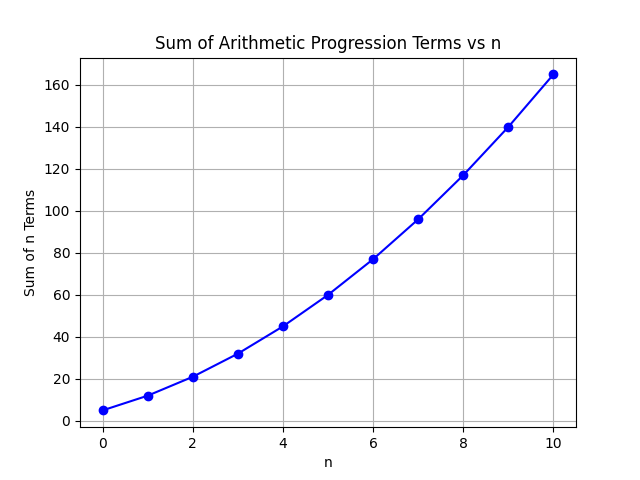
\includegraphics[width=\columnwidth]{figs/Figure_1.png}
    \caption{Plot of x(n) $vs$ n}
    \label{fig:11.9.2.11.2}
\end{figure}
\begin{table}[ht]
    \centering
    \def\arraystretch{1.5}
    \begin{tabular}{|p{4.5cm}|p{4.5cm}|}
    \hline
      $$x\brak{0}$$ & $$5$$  \\ \hline
      $$d$$ & $$2$$  \\ \hline
      $$p$$ & $$8$$  \\ \hline
      $$q$$ & $$10$$  \\ \hline
      $$r$$ & $$4$$  \\ \hline
      $$a$$ & $$96$$  \\ \hline
      $$b$$ & $$140$$  \\ \hline
      $$c$$ & $$32$$  \\ \hline
\end{tabular}
    \caption{Verified Values}
    \label{tab:11.9.2.11.3}
\end{table}
\end{document}